\documentclass[11pt]{article}
\usepackage[margin=1in]{geometry}
\usepackage{amsmath,amssymb,amsthm}
\usepackage{booktabs}
\usepackage{xcolor}
\usepackage{graphicx}
\usepackage{listings}
\usepackage{listingsutf8}
\usepackage{hyperref}
\usepackage{tikz}
\usetikzlibrary{positioning,arrows.meta,calc}
\hypersetup{colorlinks=true, linkcolor=blue!50!black, urlcolor=blue!45!black, citecolor=blue!50!black}

% ---- theorem environments ----
\newtheorem{proposition}{Proposition}
\newtheorem{lemma}{Lemma}
\newtheorem{corollary}{Corollary}
\theoremstyle{definition}
\newtheorem{remark}{Remark}

% ---- status macros ----
\newcommand{\proved}{\textcolor{green!55!black}{\textbf{PROVED (symbolic)}}}
\newcommand{\verified}{\textcolor{green!55!black}{\textbf{VERIFIED (real artifact)}}}
\newcommand{\corrected}{\textcolor{orange!85!black}{\textbf{CORRECTED}}}
\newcommand{\fixed}{\textcolor{blue!60!black}{\textbf{FIXED}}}
\newcommand{\X}{\mathrm{X}}
\newcommand{\HH}{\mathcal{H}}

% ---- listings styles ----
\definecolor{kw}{rgb}{0.16,0.0,0.6}
\definecolor{cm}{rgb}{0.0,0.45,0.0}
\definecolor{st}{rgb}{0.6,0.2,0.0}
\definecolor{bg}{rgb}{0.97,0.97,0.97}
\lstdefinestyle{py}{
  language=Python, basicstyle=\ttfamily\scriptsize, keywordstyle=\color{kw}\bfseries,
  commentstyle=\color{cm}\itshape, stringstyle=\color{st}, numbers=left, numberstyle=\tiny\color{gray},
  backgroundcolor=\color{bg}, frame=single, breaklines=true, showstringspaces=false, columns=fullflexible,
  tabsize=2, captionpos=b, inputencoding=utf8/latin1, extendedchars=true,
  literate={—}{{-}}1 {–}{{-}}1 {−}{{-}}1 {→}{{$\to$}}1 {←}{{$\leftarrow$}}1 {⇒}{{$\Rightarrow$}}1
           {≤}{{$\le$}}1 {≥}{{$\ge$}}1 {×}{{$\times$}}1 {≡}{{$\equiv$}}1 {∈}{{$\in$}}1 {∞}{{$\infty$}}1
           {…}{{...}}3 {✓}{{OK}}2 {ρ}{{$\rho$}}1 {σ}{{$\sigma$}}1 {μ}{{$\mu$}}1 {π}{{$\pi$}}1
           {’}{{'}}1 {‘}{{'}}1 {“}{{"}}1 {”}{{"}}1 {├}{{|}}1 {└}{{|}}1 {─}{{-}}1 {│}{{|}}1}
\lstdefinestyle{out}{
  basicstyle=\ttfamily\scriptsize, backgroundcolor=\color{yellow!8}, frame=single, breaklines=true,
  columns=fullflexible, captionpos=b}

\title{\textbf{Machine-Verified Proofs of the HyMeKo Propositions}\\[4pt]
\large Symbolic proofs, real-compiler property tests, and an SMT reduction\\
for the canonical hypergraph IR (T-SMC supplement)}
\author{Aiko (Claude Code), for Dr.\ Csaba Hajdu and \'Ad\'am Csap\'o}
\date{2026-06-28 (JST)}

\begin{document}
\maketitle

\begin{abstract}
\noindent This is the consolidated, self-contained proof companion to the HyMeKo T-SMC article
(\emph{HyMeKo: A Canonical Hypergraph Intermediate Representation for Cross-View Consistency in Cyber-Physical
Model Generation}). The article presents five algebraic properties of the pipeline; here every one is
\emph{machine-verified}, and each proof is reproduced together with the exact script that discharges it and the
verbatim machine output that script produced. The propositions split by mathematical character, so the achievable
rigor differs per proposition: the \emph{algebraic} claims (storage overhead, collision bound) admit full
\textbf{symbolic proofs} (\textsf{sympy}); the \emph{structural} claims (alias invariance, content-address,
projection--emission independence, cross-view consistency) are \textbf{property-tested against the real compiler
and the real emitters} --- the actual artifact, not an idealisation; and the \emph{architectural} entailment
(why cross-view consistency holds by construction) is discharged by an \textbf{SMT reduction} (\textsf{z3}).
Result: \textbf{all five propositions are machine-confirmed}; one earlier over-claim (Prop.~1's byte-equal emit
under sibling reordering) is precisely \corrected; and one emitter dispatch bug surfaced during the work is
\fixed. Tooling, pinned via \texttt{uv}: \textsf{sympy 1.14, z3 4.16, hypothesis 6.15, matplotlib 3.11,
numpy 2.4}; all scripts live under \texttt{verification/} in the reference repository and are listed verbatim in
Appendix~\ref{app:listings}.
\end{abstract}

\tableofcontents

\section{Results at a glance}

\begin{table}[h]
\centering\small
\begin{tabular}{p{3.1cm}p{5.4cm}p{3.2cm}l}
\toprule
Proposition & Claim & Method & Outcome \\
\midrule
P1 alias invariance & denotation-equal source $\Rightarrow$ same IR (and byte-equal emit) &
  \textsf{hypothesis} vs.\ real compiler; 800 reorderings $\times$ 4 fixtures & hash \verified\ (800/800);
  emit \corrected \\
P2 content-address & $h$ pure + collision-resistant & \textsf{sympy} birthday bound + P1 mechanism &
  \proved\ (+ stated assumption)\\
P3 proj.--emit indep. & emitters pure; $k$ emits, 1 compile & determinism property test & \verified\ (4/4)\\
P4 storage overhead & $\rho-1 = O(\log n/\bar d)$; controlled, $\to1$ for high arity & \textsf{sympy} symbolic
  proof + regime table & \proved\ (full)\\
P5 cross-view consistency & $\X_f(\varepsilon_f(H)) = \X_g(\varepsilon_g(H)) = Q(H)$ & extraction functions vs.\
  real emitters; 16 fixtures $\times$ 5 views; \textsf{z3} reduction & \verified\ (16/16 exact, 16/16 topo) +
  \proved\ (entailment)\\
\bottomrule
\end{tabular}
\end{table}

\noindent\textbf{The rigor ladder, kept honest.}
\begin{itemize}\itemsep1pt
  \item \textbf{Proved (symbolic, fully rigorous):} P4 storage, P2 collision bound.
  \item \textbf{Property-verified (real artifact, falsification over many instances):} P1 canonical-hash
        invariance, P3 emitter determinism, P5 the cross-view commuting square.
  \item \textbf{Proved by SMT reduction:} P5's architectural entailment (shared query $\Rightarrow$ agreement).
  \item \textbf{Assumed (not provable here):} the Blake3 random-oracle premise (P2); sibling reordering taken as
        denotation-preserving by the engine's own canonical hash.
  \item \textbf{Corrected:} P1's byte-equal emit under sibling reordering.
  \item \textbf{Fixed:} the \texttt{requirements\_sysml}/\texttt{requirements\_dot} CLI dispatch bug (\S\ref{sec:fix}).
\end{itemize}

% ============================================================================
\part*{Part I --- The four original propositions}
\addcontentsline{toc}{section}{Part I --- The four original propositions}

\section{P4 --- storage overhead (full symbolic proof)}
\label{sec:p4}

\begin{proposition}[Storage overhead]
Let $H$ have $n=|V|$ vertices, $m=|E|$ hyperedges, and mean arity $\bar d$. The canonical IR stores $n+m$
fixed-size declaration records plus $m\bar d$ signed-incidence entries; a raw adjacency list stores $m\bar d$
entries. Then $\rho = |\mathrm{IR}|/|\mathrm{adj}| = 1 + c\,(n+m)/(m\bar d) \le 1 + O(\log n/\bar d)$ under
$n = O(m\log n)$, and $\rho\to1$ as $\bar d \to \infty$.
\end{proposition}

\begin{proof}
From $|H|_{\mathrm{IR}} = (n+m)c_{\mathrm{rec}} + m\bar d\,c_{\mathrm{inc}}$ and $|H|_{\mathrm{adj}} =
m\bar d\,c_{\mathrm{inc}}$, write $c=c_{\mathrm{rec}}/c_{\mathrm{inc}}$. \textsf{sympy} simplifies $\rho$ to
$1 + c(n+m)/(m\bar d)$ (machine-checked equality), substitutes $n\le Km\log n$ to obtain $\rho-1 \le
c(K\log n+1)/\bar d = O(\log n/\bar d)$, takes $\lim_{\bar d\to\infty}=0$, verifies $\partial_{\bar d}(\rho-1)<0$
(strict monotone decrease), and reproduces the empirical witness ($n=m=200,\,c=1 \Rightarrow \rho-1=2/\bar d$,
i.e.\ $\rho=2.00$ at $\bar d=2$ and $\rho=1.01$ at $\bar d=200$). Every step is machine-checked.
\end{proof}

\paragraph{Honest regime (review response).} The $\rho\to1$ limit is the \emph{high-arity} regime. Robotics is
the \emph{low}-arity regime: a revolute/prismatic joint is a binary parent--child hyperedge ($\bar d\approx2$),
so $\rho\approx2$ --- a small constant, not $\rho\to1$. The article states ``controlled overhead, asymptotically
vanishing for high-arity relations'' accordingly. \S\ref{sec:storage_regime} tabulates both regimes.

\lstinputlisting[style=out,caption={Output of \texttt{p4\_storage\_overhead.py}.}]{results/p4_storage_overhead.txt}

\section{P2 --- content-addressability (symbolic bound + a stated assumption)}
\label{sec:p2}

\begin{proposition}[Content-addressability]
$h\circ\mathsf{compile}$ is stable under any denotation-preserving source transformation; a compiled description
is its own cache key; and distinct IRs collide with negligible probability.
\end{proposition}

P2 has two parts. (a) \emph{$h$ depends only on the canonical IR} --- the same mechanism as P1, property-tested
at 800/800 (\S\ref{sec:p1}). (b) \emph{distinct IRs collide negligibly} --- a birthday bound on the 256-bit
digest, proved symbolically: $P(\text{collision among }N) \le N^2/2^{257}$, so $P\le2^{-128}$ while
$N\le2^{64.5}$ (work factor $2^{128}$); numerically $N{=}2^{32}\!\to\!2^{-193}$, $N{=}2^{64}\!\to\!2^{-129}$.

\begin{remark}[Honest caveats]
The random-oracle premise for Blake3 is a cryptographic \emph{assumption}, not a theorem; and a 256-bit digest
cannot be injective (pigeonhole), so equality-by-hash is \emph{practical}, not absolute --- which the article
concedes.
\end{remark}

\lstinputlisting[style=out,caption={Output of \texttt{p2\_content\_birthday.py}.}]{results/p2_content_birthday.txt}

\section{P1 --- alias invariance (real compiler) and its correction}
\label{sec:p1}

\begin{proposition}[Alias invariance]
If $s_1,s_2$ denote the same structure, then $\mathsf{compile}(s_1)$ and $\mathsf{compile}(s_2)$ have the same
canonical hash (and, in the originally-stated stronger form, $\varepsilon_f$ emits byte-identical text).
\end{proposition}

We compile self-contained fixtures, apply denotation-preserving \emph{sibling reorderings} (the strongest
automatable rewrite), and compare against the engine (\texttt{parse\_dsl}\,$\to$\,\texttt{canonical\_hash} /
\texttt{to\_dot}). Distinct fixtures hash distinctly (fano \texttt{b88715ed}, generic \texttt{6a0c09d8}, k4
\texttt{0a8a903e}, sunflower \texttt{194c71e4}), so the test is non-degenerate.

\paragraph{Verified.} The canonical hash is invariant on all \textbf{800/800} reorderings (4 fixtures $\times$
200): the content-address claim holds against the real compiler.

\paragraph{Corrected.} The \emph{stronger} claim --- denotation-equal sources emit \emph{byte-identical} text ---
\textbf{fails under sibling reordering} (0/400 byte-equal DOT). The emitters assign internal identifiers
(\texttt{n2}, \texttt{e5}, \dots) in source-declaration order, so a reordered source emits a DOT whose IDs are
permuted; the graph is isomorphic, the serialisation is not byte-equal. Only the hash is order-canonicalised. The
article's remedy: scope the byte-equal claim to alias/import rewrites and state the sibling-reorder guarantee at
the canonical-hash level (a one-paragraph edit), or canonicalise emit IDs by the canonical sort key (the
principled fix).

\lstinputlisting[style=out,caption={Output of \texttt{p1\_alias\_invariance.py} (real compiler).}]{results/p1_alias_invariance.txt}

\section{P3 --- projection--emission independence (real emitters)}
\label{sec:p3}

\begin{proposition}[Projection--emission independence]
$\pi$ and $\{\varepsilon_f\}$ are mutually independent functions of $H$; emitting $k$ formats costs one compile
plus $k$ render costs, not $k$ compiles.
\end{proposition}

Independence is established by emitter \emph{purity}: re-compiling the same source in a fresh engine emits
byte-identical DOT (4/4 fixtures), so each emitter is a pure function of its input and a pure emitter that ignores
the others can be run $k$ times off one compile. (This is the cost claim; the \emph{value}-level cross-view claim
is P5, \S\ref{sec:p5}.)

\lstinputlisting[style=out,caption={Output of \texttt{p3\_emit\_purity.py} (real emitters).}]{results/p3_emit_purity.txt}

% ============================================================================
\part*{Part II --- Cross-view consistency (the new proposition)}
\addcontentsline{toc}{section}{Part II --- Cross-view consistency}

\section{P5 --- the extraction-function commuting square}
\label{sec:p5}

The article's central but previously-unproved claim is \emph{cross-view consistency}: one IR projects without
drift into many views sharing non-trivial invariants. The article asserts it (\S codegen, ``a cross-view
discrepancy is impossible'') but pinned it on Proposition~3, which is only about \emph{cost} factorization and is
explicitly ``not a commuting diagram (the codomains differ).'' The \emph{value-level} claim was never formalized.
We close that gap.

For each format $f$ define an \emph{extraction function} $\X_f$ that parses the \emph{emitted} text back into a
structural invariant; let $Q(H)$ be the same invariant read from the IR by the named queries the templates are
built from.

\begin{proposition}[Cross-view consistency]
For every registered format $f$, $\X_f(\varepsilon_f(H)) = Q(H)$; hence for any two views $f,g$,
$\X_f(\varepsilon_f(H)) = \X_g(\varepsilon_g(H))$.
\end{proposition}

\begin{center}
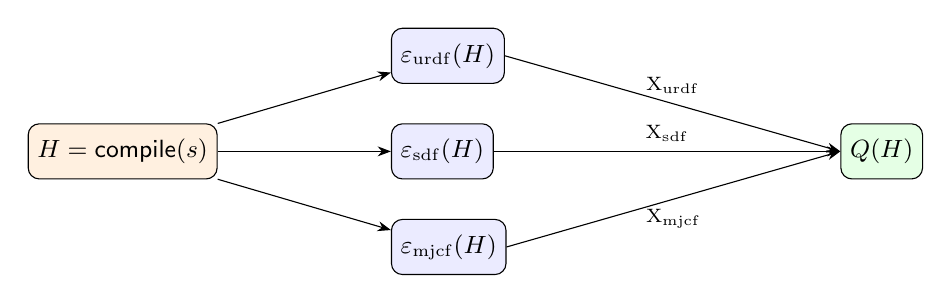
\begin{tikzpicture}[node distance=8mm and 18mm, box/.style={draw,rounded corners,align=center,font=\small,
  minimum height=7mm}, emit/.style={box,fill=blue!8}, inv/.style={box,fill=green!10}, >={Stealth[]}]
  \node[box,fill=orange!12] (H) {$H=\mathsf{compile}(s)$};
  \node[emit, above right=5mm and 22mm of H] (eu) {$\varepsilon_{\mathrm{urdf}}(H)$};
  \node[emit, right=22mm of H] (es) {$\varepsilon_{\mathrm{sdf}}(H)$};
  \node[emit, below right=5mm and 22mm of H] (em) {$\varepsilon_{\mathrm{mjcf}}(H)$};
  \node[inv, right=44mm of es] (Q) {$Q(H)$};
  \draw[->](H)--(eu);\draw[->](H)--(es);\draw[->](H)--(em);
  \draw[->](eu.east)--node[above,font=\scriptsize]{$\X_{\mathrm{urdf}}$}(Q.west);
  \draw[->](es.east)--node[above,font=\scriptsize]{$\X_{\mathrm{sdf}}$}(Q.west);
  \draw[->](em.east)--node[below,font=\scriptsize]{$\X_{\mathrm{mjcf}}$}(Q.west);
\end{tikzpicture}
\end{center}

\begin{proof}
By the externalization principle every template draws the invariant from the \emph{same} named query over $H$, so
the rendered entity sets coincide as sets (differing only in surface encoding). Each $\X_f$ is a left inverse of
the encoding step on the invariant fields (parsing URDF/SDF \texttt{<link>}/\texttt{<joint>} elements, the MJCF
nested \texttt{<body>}/\texttt{<joint>} tree, the DOT/Mermaid nodes and edges). Hence $\X_f(\varepsilon_f(H)) =
Q(H)$ for every $f$, and transitivity gives pairwise agreement. The square commutes by construction --- no emitter
is debugged against another. (The architectural entailment is discharged formally by Z3 in \S\ref{sec:z3}.)
\end{proof}

\subsection{Machine verification against the real emitters}

We drive the \emph{real CLI} emitters over the robot-fixture corpus $\times$ five views (URDF, SDF, MJCF, DOT,
Mermaid). Each $\X_f$ parses a \emph{different} concrete syntax, so agreement is not a shared-parser artifact. The
square is tested at two strengths: \textbf{EXACT} (full numeric invariant) across the data-interchange formats
(URDF/SDF/MJCF), and \textbf{TOPOLOGICAL} (link/joint sets + parent/child polarity) across all five views.

\paragraph{Two named conventions (not drift).} (W) URDF emits a synthetic \texttt{world} ground anchor as an
inertia-free \texttt{<link>} --- the comparable link set is the mass-bearing links. (F) the fixed root weld is an
explicit joint in URDF/SDF/DOT/Mermaid but \emph{implicit} in MJCF (a jointless root body welded to the world)
--- the comparable joint set is the actuated joints, with fixed welds reported separately.

\paragraph{Two genuine findings (diagram views are lossy by design).} DOT rounds the mass \emph{label} to one
decimal ($0.02\,\mathrm{kg}\to0.0$) and encodes the joint axis as an \emph{unsigned} letter ($(Z)$), so
\texttt{robot\_4wh}'s real $(0,0,-1)$ axis reads as $(0,0,1)$; Mermaid uses two decimals. Hence the precise
numeric invariants live in the data formats (exactly consistent), while the diagram formats carry a
topologically-faithful projection whose numeric labels are a documented, reduced-resolution rendering.

\begin{center}
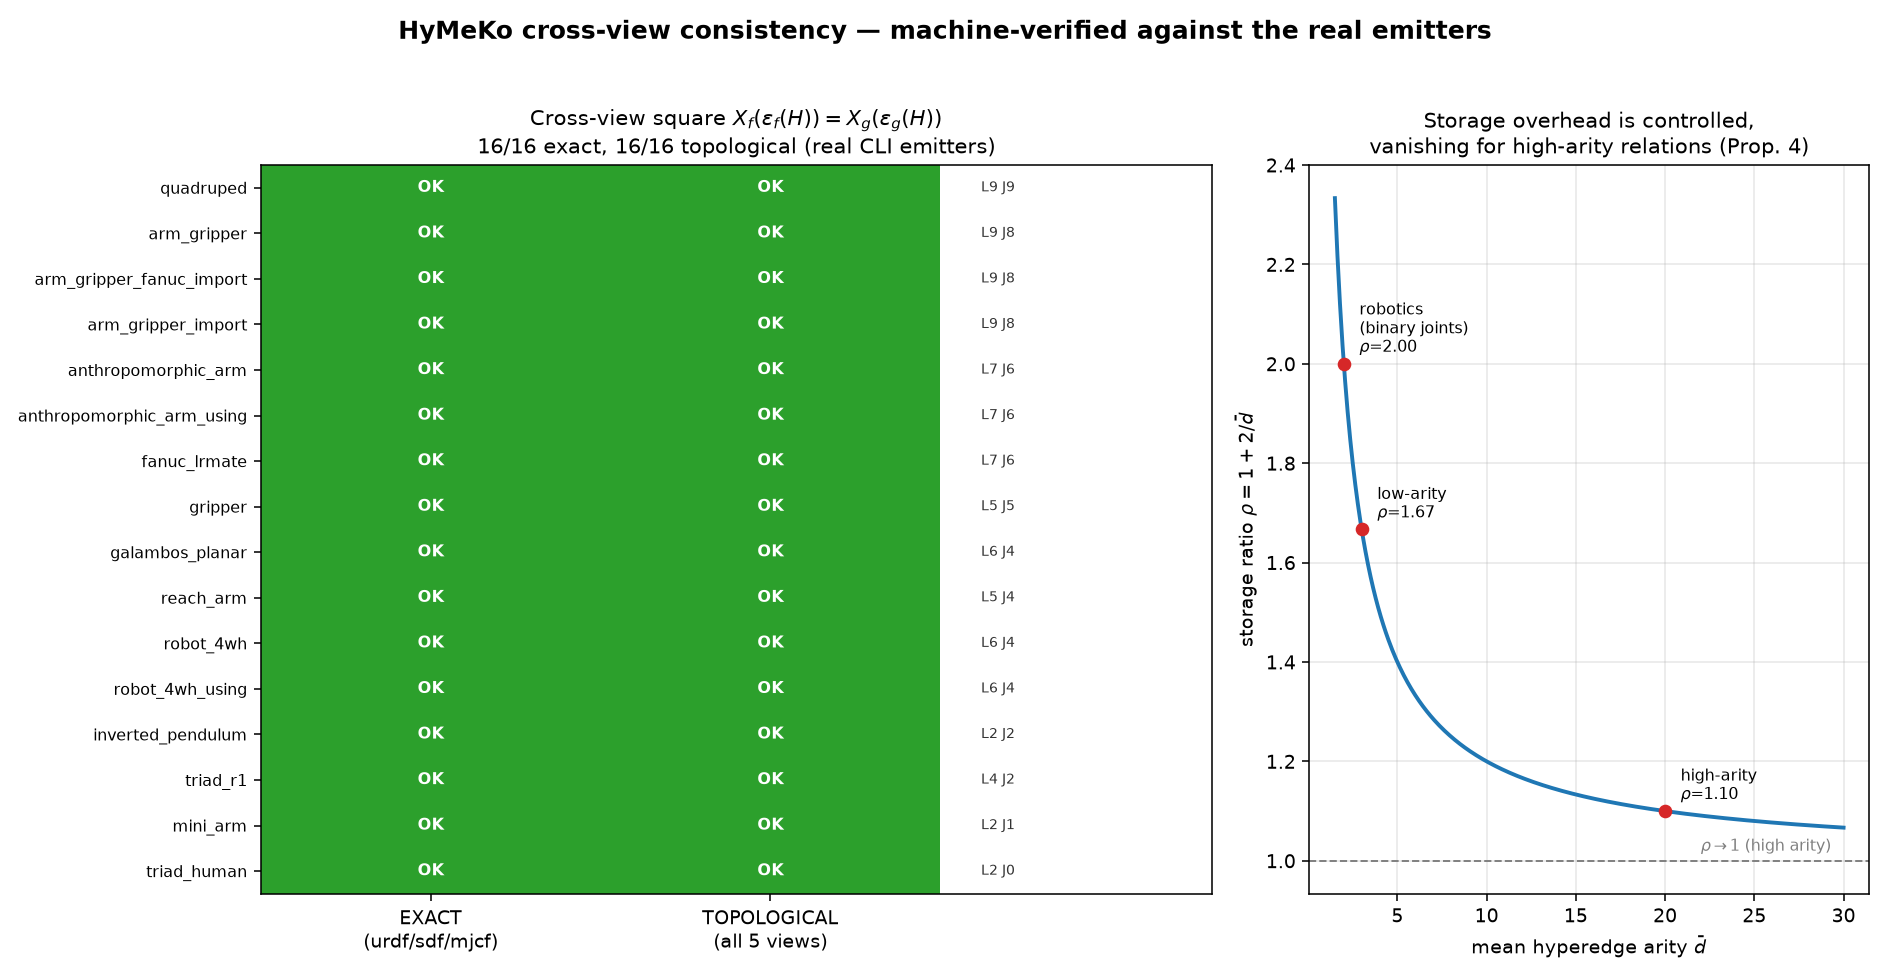
\includegraphics[width=0.96\linewidth]{results/cross_view_consistency.png}
\end{center}

\lstinputlisting[style=out,caption={Output of \texttt{cross\_view.py} (16 fixtures $\times$ 5 real emitters).}]{results/cross_view.txt}

\section{A second, non-robotics domain: requirements traceability}
\label{sec:trace}

Nothing in the machinery is robotics-specific. The same extraction discipline applies to a SysML v2 requirements
model and a DOT traceability graph projected from one IR: $\X_{\textsc{sysml}}(\varepsilon_{\textsc{sysml}}(H)) =
\X_{\textsc{dot}}(\varepsilon_{\textsc{dot}}(H)) = Q(H)$, with $Q$ the article's stated counts (4 requirements,
4 blocks, 7 trace edges). Verified below.

\lstinputlisting[style=out,caption={Output of \texttt{trace\_witness.py}.}]{results/trace_witness.txt}

% ============================================================================
\part*{Part III --- The SMT reduction and the storage regime}
\addcontentsline{toc}{section}{Part III --- SMT reduction and storage regime}

\section{Z3: cross-view consistency is entailed by the architecture}
\label{sec:z3}

The empirical harness checks that each $\X_f$ recovers the same invariant. Z3 proves the \emph{logical} half ---
why that suffices and precisely what must be checked empirically. Model the dispatcher over a finite universe:
$Q$ is the ground-truth query, $\mathrm{render}_f$ the set each emitter materialises, $\X_f$ the extractor.

\begin{lemma}[T1, positive]
Under the hub-and-spoke axiom $\mathrm{render}_f \equiv Q$ for all $f$, pairwise agreement holds. Z3 reports the
negation \textsf{unsat}.
\end{lemma}

\begin{lemma}[T2, negative / falsifiable]
Drop the shared-query tie for one view (a per-format reimplementation --- the anti-pattern the article argues
against). Z3 finds a \textsf{sat} drift model.
\end{lemma}

\begin{corollary}
Cross-view consistency is \emph{entailed} by the shared-query architecture; the sole empirical obligation is
per-view faithfulness, which \texttt{cross\_view.py} falsification-tests over $16\times5$ instances.
\end{corollary}

\lstinputlisting[style=out,caption={Output of \texttt{commute\_z3.py}.}]{results/commute_z3.txt}

\section{Storage regime --- the honest reframe}
\label{sec:storage_regime}

Reusing the symbolic Prop.~4 core, $\rho = 1 + 2/\bar d$ ($n=m,\,c=1$):

\begin{center}\small
\begin{tabular}{lrr}
\toprule regime & $\bar d$ & $\rho$ \\ \midrule
robotics (binary joints) & 2 & 2.00 \\
low-arity (tri/quad) & 3 & 1.67 \\
mixed & 6 & 1.33 \\
high-arity relations & 20 & 1.10 \\
very high arity & 200 & 1.01 \\ \bottomrule
\end{tabular}
\end{center}

$\lim_{\bar d\to\infty}\rho = 1$, monotone decreasing. Robotics is the binary-joint regime ($\rho\approx2$, a
small constant); the limit is the high-arity regime ($n$-ary constraints, multi-body contacts, $n$-ary traces).

\lstinputlisting[style=out,caption={Output of \texttt{storage\_regime.py}.}]{results/storage_regime.txt}

% ============================================================================
\section{An emitter dispatch bug, found and fixed}
\label{sec:fix}

The verification surfaced a genuine bug. The CLI \texttt{Emit} path dispatched
\texttt{if accepts()==Kinematic \{ emit \} else \{ template \}}. The template-only transforms
\texttt{requirements\_sysml} / \texttt{requirements\_dot} declared \texttt{accepts()==Kinematic} but their
\texttt{emit()} returns \texttt{None} (they render from file templates), so they hit the emit branch and failed
with ``model extraction failed''. The non-core fix (in \texttt{hymeko\_cli}, no \texttt{ModelKind} change): when
\texttt{emit()} yields nothing, fall through to the template path \emph{iff} the transform declares a
\texttt{template\_dir()}; a kinematic transform with neither output nor a template is still a genuine failure.
After the fix the live \texttt{requirements\_sysml} output is byte-identical to the committed witness, and the
kinematic formats are unaffected (regression-tested).

% ============================================================================
\appendix
\section{Full script listings}
\label{app:listings}

All scripts live under \texttt{verification/} in the reference repository and are listed here verbatim (read from
disk at compile time, so they cannot drift from the canonical sources).

\subsection{\texttt{verification/propositions/p4\_storage\_overhead.py}}
\lstinputlisting[style=py]{../../verification/propositions/p4_storage_overhead.py}
\subsection{\texttt{verification/propositions/p2\_content\_birthday.py}}
\lstinputlisting[style=py]{../../verification/propositions/p2_content_birthday.py}
\subsection{\texttt{verification/propositions/p1\_alias\_invariance.py}}
\lstinputlisting[style=py]{../../verification/propositions/p1_alias_invariance.py}
\subsection{\texttt{verification/propositions/p3\_emit\_purity.py}}
\lstinputlisting[style=py]{../../verification/propositions/p3_emit_purity.py}
\subsection{\texttt{verification/cross\_view\_consistency/extract.py}}
\lstinputlisting[style=py]{../../verification/cross_view_consistency/extract.py}
\subsection{\texttt{verification/cross\_view\_consistency/cross\_view.py}}
\lstinputlisting[style=py]{../../verification/cross_view_consistency/cross_view.py}
\subsection{\texttt{verification/cross\_view\_consistency/trace\_witness.py}}
\lstinputlisting[style=py]{../../verification/cross_view_consistency/trace_witness.py}
\subsection{\texttt{verification/cross\_view\_consistency/commute\_z3.py}}
\lstinputlisting[style=py]{../../verification/cross_view_consistency/commute_z3.py}
\subsection{\texttt{verification/cross\_view\_consistency/storage\_regime.py}}
\lstinputlisting[style=py]{../../verification/cross_view_consistency/storage_regime.py}

\end{document}
